% Talk outline
% Want to tell you about Disco.
% Goals of disco
% - Teach FP concepts.
%   - At small institution, don't have luxury of
%     teaching intro FP.
%   - Idea of teaching FP + Discrete is not at all new.
% - Connect math & computation
% - Enhance learning
% - Minimize friction.  Many existing approaches use a
%   general-purpose functional language.  But let's talk about that.
% Show example function.
% Haskell implementation:
% - Int/Rational instead of N/Q
% - Can't match on 2n, 2n+1.  Can't write 3n.
% - Have to convert Int to Rational with fromIntegral
% Show Disco implementation.
%   Anecdotally, this works.  Students were able to use it with very
%   little issue.

% Demo
% First, show calculator.  Addition, subtraction, mult, big power
% (arbitrary sized integers), division (fractions)
% Show types of things.  Subtyping.  :type [1,-2,1/3]
% Show subtyping diamond (on slides).
% Back to demo.
% - Show gcd.  Talk about docs, tests, randomized property-based
%   testing.
% - Show zorder. each(zOrder', [0..15])
% - Show module6, using properties to create an assignment.  Exercise
%   4.
% - Show catalan.  Algebraic types, equirecursive types.  Great way
%   to introduce students to algebraic data types.

% Then talk about issues / future work.  Take more or less time as needed.

% -*- mode: LaTeX; compile-command: "rubber --unsafe -d disco-tfpie23-talk.tex" -*-

\documentclass[fleqn,xcolor={usenames,dvipsnames,svgnames,table},12pt,aspectratio=169]{beamer}

%%%%%%%%%%%%%%%%%%%%%%%%%%%%%%%%%%%%%%%%%%%%%%%%%%%%%%%%%%%%
%% Beamer setup
%%%%%%%%%%%%%%%%%%%%%%%%%%%%%%%%%%%%%%%%%%%%%%%%%%%%%%%%%%%%

\mode<presentation>
{
  \usetheme{default}                          % use a default (plain) theme

  \setbeamertemplate{navigation symbols}{}    % don't show navigation
                                              % buttons along the
                                              % bottom
  \setbeamerfont{normal text}{family=\sffamily}

%  \setbeamertemplate{footline}[frame number]

  \AtBeginSection[]
  {
    \begin{frame}<beamer>
      \frametitle{}
      \begin{center}
        {\Huge \insertsectionhead}

        \vspace{0.25in}
        \includegraphics[width=2in]{\secimage}
      \end{center}
    \end{frame}
  }
}

% \newcommand{\secimage}{yuk.jpg}

\newenvironment{xframe}[1][]
  {\begin{frame}[fragile,environment=xframe,#1]}
  {\end{frame}}

% uncomment me to get 4 slides per page for printing
% \usepackage{pgfpages}
% \pgfpagesuselayout{4 on 1}[uspaper, border shrink=5mm]

% \setbeameroption{show only notes}

%%%%%%%%%%%%%%%%%%%%%%%%%%%%%%%%%%%%%%%%%%%%%%%%%%%%%%%%%%%%
%% Package imports
%%%%%%%%%%%%%%%%%%%%%%%%%%%%%%%%%%%%%%%%%%%%%%%%%%%%%%%%%%%%

\usepackage[english]{babel}
\usepackage[T1]{fontenc}
\usepackage{graphicx}
\graphicspath{{images/}{../../../images/}}

\usepackage{ulem}
\usepackage{url}
\usepackage{fancyvrb}
\usepackage{xspace}
\usepackage{minted}

%%%%%%%%%%%%%%%%%%%%%%%%%%%%%%%%%%%%%%%%%%%%%%%%%%%%%%%%%%%%
%% Semantic markup
%%%%%%%%%%%%%%%%%%%%%%%%%%%%%%%%%%%%%%%%%%%%%%%%%%%%%%%%%%%%

\newcommand{\disco}{\textsc{Disco}\xspace}

\newcommand{\term}[1]{\emph{#1}}

\newcommand{\pkg}[1]{\href{https://hackage.haskell.org/package/#1}{\texttt{#1}}}
\newcommand{\ext}[1]{\texttt{#1}}
\newcommand{\module}[1]{\texttt{#1}}

\newcommand{\ie}{\emph{i.e.}\ }
\newcommand{\eg}{\emph{e.g.}\ }
\newcommand{\etal}{\emph{et al.}\xspace}
\newcommand{\etc}{\emph{etc.}\xspace}

%%%%%%%%%%%%%%%%%%%%%%%%%%%%%%%%%%%%%%%%%%%%%%%%%%
% Notes
%%%%%%%%%%%%%%%%%%%%%%%%%%%%%%%%%%%%%%%%%%%%%%%%%%

\newif\ifcomments\commentsfalse

\ifcomments
\newcommand{\authornote}[3]{\textcolor{#1}{[#3 ---#2]}}
\newcommand{\todo}[1]{\textcolor{red}{[TODO: #1]}}
\else
\newcommand{\authornote}[3]{}
\newcommand{\todo}[1]{}
\fi

\newcommand{\brent}[1]{\authornote{blue}{BAY}{#1}}

%%%%%%%%%%%%%%%%%%%%%%%%%%%%%%%%%%%%%%%%%%%%%%%%%%%%%%%%%%%%
%% Math typesetting
%%%%%%%%%%%%%%%%%%%%%%%%%%%%%%%%%%%%%%%%%%%%%%%%%%%%%%%%%%%%

\newcommand{\N}{\mathbb{N}}
\newcommand{\Z}{\mathbb{Z}}
\newcommand{\F}{\mathbb{F}}
\newcommand{\Q}{\mathbb{Q}}

\DeclareUnicodeCharacter{27C5}{$\Lbag$}
\DeclareUnicodeCharacter{27C6}{$\Rbag$}
\DeclareUnicodeCharacter{2192}{$\to$}
\DeclareUnicodeCharacter{D7}{$\times$}
\DeclareUnicodeCharacter{2200}{$\forall$}
\DeclareUnicodeCharacter{2115}{$\N$}
\DeclareUnicodeCharacter{2124}{$\Z$}
\DeclareUnicodeCharacter{211A}{$\Q$}
\DeclareUnicodeCharacter{1D53D}{$\F$}
\DeclareUnicodeCharacter{03BB}{$\lambda$}

%%%%%%%%%%%%%%%%%%%%%%%%%%%%%%%%%%%%%%%%%%%%%%%%%%%%%%%%%%%%
%% Title
%%%%%%%%%%%%%%%%%%%%%%%%%%%%%%%%%%%%%%%%%%%%%%%%%%%%%%%%%%%%

\title{\disco \\ \small{A Functional Programming Language for Discrete
  Matheamtics} \\ \bigskip \includegraphics[width=0.75in]{logo.png}}
\date{TFPIE 2023, Boston}
\author{Brent A. Yorgey, Hendrix College}
\titlegraphic{}

%%%%%%%%%%%%%%%%%%%%%%%%%%%%%%%%%%%%%%%%%%%%%%%%%%%%%%%%%%%%%%%%%%%

\begin{document}

\maketitle

\begin{frame}{\disco}
  \begin{center}\includegraphics[width=0.75in]{logo.png}\end{center}

  \begin{itemize}
  \item Functional teaching language
  \item Designed for use in a Discrete Mathematics course
  \item Birthplace: TFPIE 2016, Maryland, USA!
  \item Have used it in a Discrete Math class once, in
    Spring 2022.
  \item Plan to use it again starting next week.
  \end{itemize}
\end{frame}

\begin{frame}{\disco goals}
  \begin{itemize}
  \item Teach early CS students basic FP concepts
  \item Help students connect math and computation
  \item Enhance learning with an interactive platform
  \item Minimize notational \& conceptual friction
  \end{itemize}
\end{frame}

\begin{xframe}{Friction?}
  \begin{align*}
    f &: \N \to \Q \\
    f(2n)   &= 0 \\
    f(2n+1) &= \begin{cases} n/2 & \text{if } n > 5, \\
      3n + 7 & \text{otherwise}
      \end{cases}
  \end{align*}

  \begin{overprint}
    \onslide<2>

    \begin{center}
  \begin{minted}{haskell}
f :: Int -> Rational
f x
  | even x    = 0
  | n > 5     = fromIntegral n / 2
  | otherwise = 3*n + 7
  where
    n = x `div` 2
  \end{minted}
    \end{center}

  \onslide<3>
  \begin{minted}{text}
f : N -> Q
f(2n)   = 0
f(2n+1) = {? n/2      if n > 5,
             3n + 7   otherwise
          ?}
  \end{minted}
  \end{overprint}
\end{xframe}

\begin{xframe}{Demo!}
  \url{https://replit.com/@BrentYorgey/Disco#README.md}
\end{xframe}

\begin{xframe}{Numeric types in \disco}
  \begin{center}
    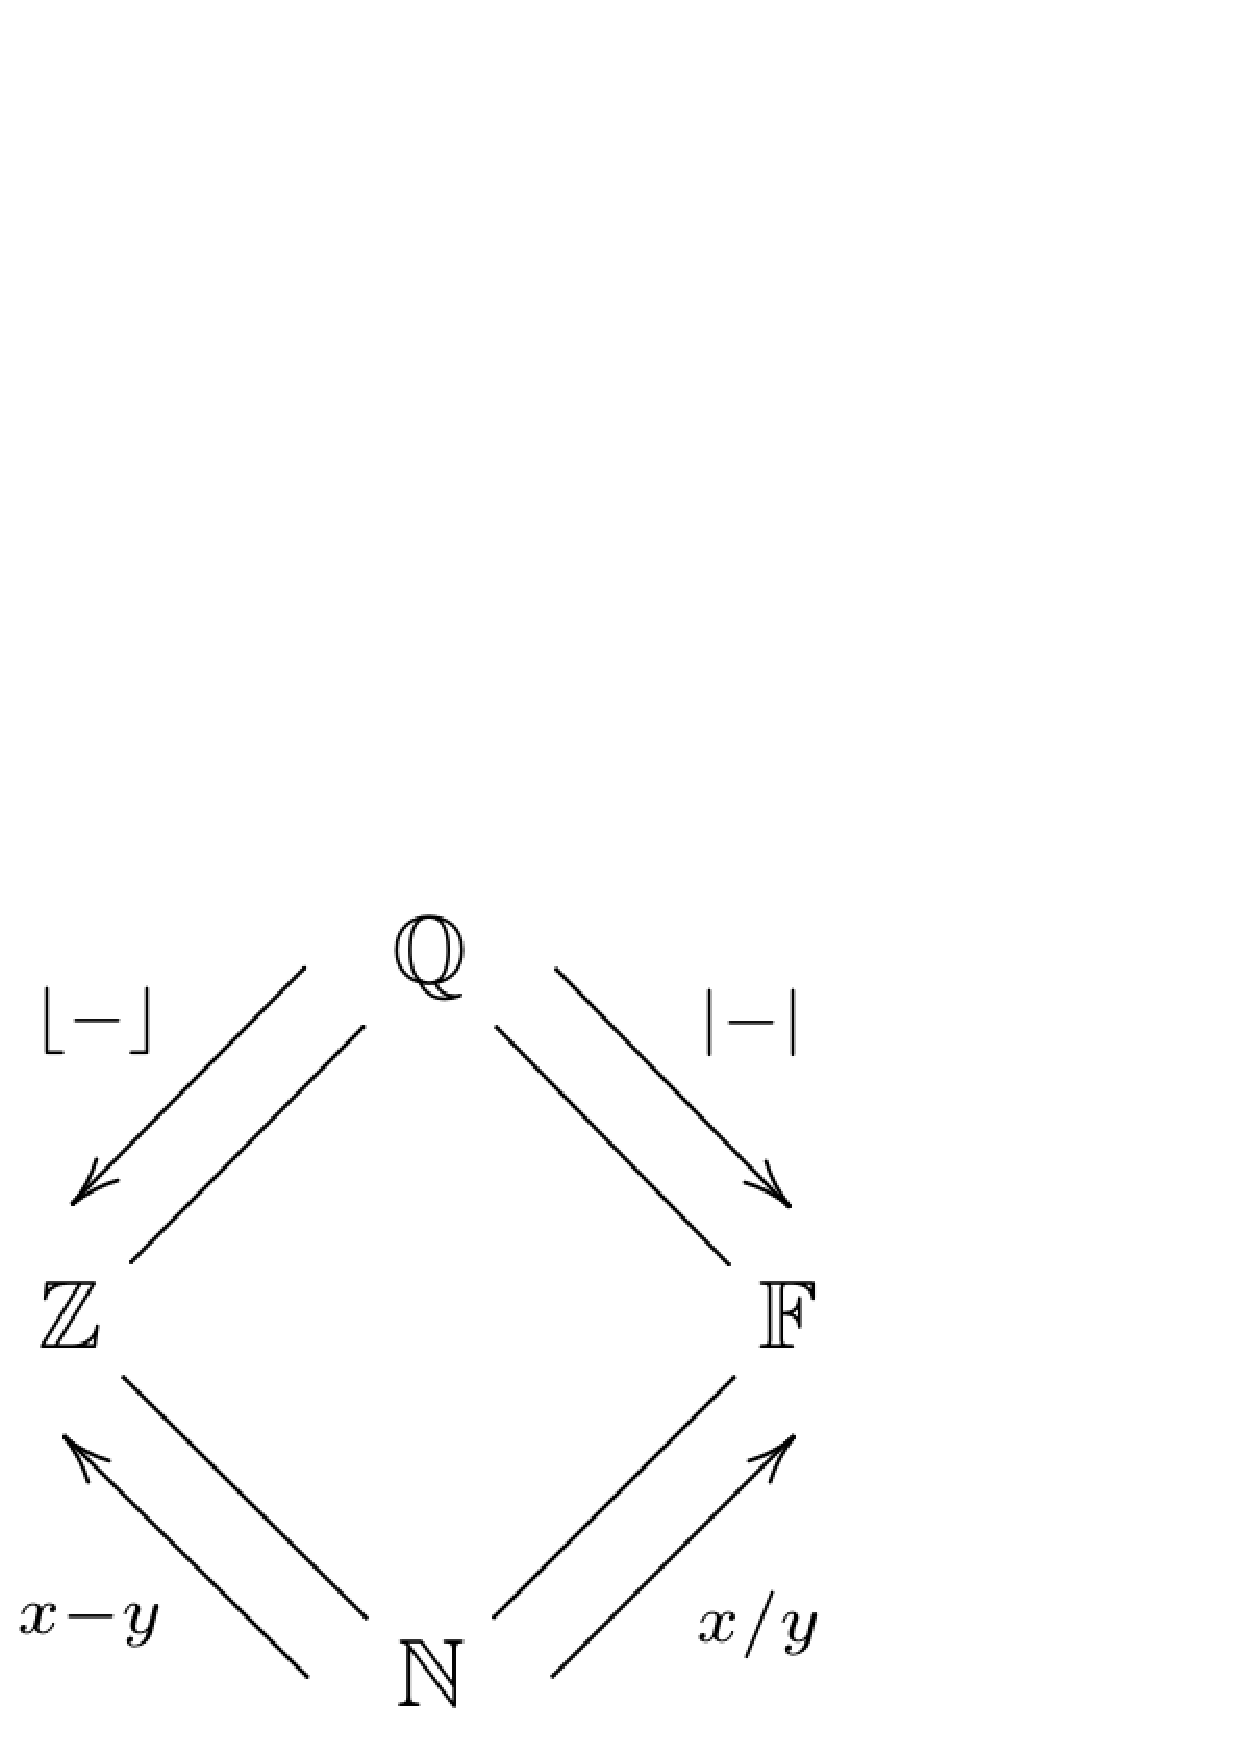
\includegraphics[width=0.3\textwidth]{../../../docs/images/diamond.png}
  \end{center}
\end{xframe}

\begin{xframe}{Issues / Future work}
  \begin{itemize}
  \item Error messages!
  \item Showing multiple type instantiations
  \item Types vs sets
  \end{itemize}
\end{xframe}

\begin{xframe}{Showing multiple type instantiations}
  What is the most general type of $\lambda x. x - 2$?
  \bigskip

  \onslide<2-> Internally, it is something like $\forall
  a. (\mathrm{HasSubtraction}(a), \Z <: a) \Rightarrow a \to a$
  \bigskip

  \onslide<3-> \dots but we definitely don't want to show that to
  students! \bigskip

  \onslide<4-> We do this instead, but it's confusing:
  \begin{verbatim}
Disco> :type \x. x - 2
λx. x - 2 : ℤ → ℤ
Disco> (\x. x - 2) (5/2)
1/2
  \end{verbatim}
\end{xframe}

\begin{xframe}{Showing multiple type instantiations}
  What about something like this instead?
  \begin{verbatim}
  Disco> :type \x. x - 2
  λx. x - 2
    : ℤ → ℤ
    : ℚ → ℚ
  \end{verbatim}
\end{xframe}

\begin{xframe}{Types vs sets}
  \begin{itemize}
  \item<+-> $\{2,4,7\}$ is an example of a \underline{\hspace{2in}}
  \item<+-> $\N$ is an example of a \underline{\hspace{2in}}
  \item<+-> In a math class, $\N - \{2,4,7\}$ is a perfectly well-defined,
  countably infinite set.
  \item<+-> In \disco, $\N - \{2,4,7\}$ is a \emph{syntax error}!
  \item<+-> Why the difference, and how do we explain/frame it for
    students??
  \end{itemize}
  \bigskip
\end{xframe}

\begin{xframe}
  \begin{center}
  \url{https://github.com/disco-lang/disco}
  \bigskip

  \includegraphics[width=0.75in]{logo.png}
  \end{center}
\end{xframe}

\end{document}
